\documentclass[12pt,a4paper,UTF8]{ctexart}
\usepackage{geometry}
	\geometry{left=2.5cm,right=2.5cm,top=2cm,bottom=2cm}
\usepackage{xeCJK,amsmath,paralist,enumitem,booktabs,multirow,graphicx,subfig,setspace}
	\setlength{\parindent}{2em}
\usepackage[colorlinks,linkcolor=blue,urlcolor=blue]{hyperref}

%%%%%%%%%%%%%%%%%%%%%%%%%正文开始%%%%%%%%%%%%%%%%%%%%%%%%%%
\begin{document}

%%%%%%%%附录:数据处理%%%%%%%
\newpage
\pagestyle{plain}
\begin{center}
\LARGE\textbf{实验B11 圆孔衍射}
\end{center}

%%信息
\begin{doublespacing}
	\centering
	\begin{tabular}{ll}
	 & \\
	{\CJKfontspec{Droid Sans Fallback} 实验人:黄子维 20980066} & {\CJKfontspec{Droid Sans Fallback}合作者:黄睿杰 20980062}\\
	{\CJKfontspec{Droid Sans Fallback} 实验时间:2021.11.4~星期四~上午} & {\CJKfontspec{Droid Sans Fallback} 室温:23$^{\circ}$C~相对湿度:78\%}
	\end{tabular}
\end{doublespacing}

\subsection*{【实验参数】}
激光波长$\lambda = 632.8nm$
\paragraph{夫琅禾费圆孔衍射}
\begin{itemize}
    \item 出光口到多孔板:19.75cm
    \item 多孔板到光探头:79.25cm
    \item 孔径:0.15mm,0.3mm,0.5mm
\end{itemize}

\paragraph{菲涅尔圆孔衍射}
\begin{itemize}
    \item 出光口到扩束镜:2.8cm
    \item 孔径 1.5mm
        \begin{itemize}
            \item 扩束镜到多孔板:16.95cm
            \item 多孔板到光探头:43.25cm,77.25cm
        \end{itemize}
    \item 孔径 1.0mm
        \begin{itemize}
            \item 扩束镜到多孔板:19.20cm
            \item 多孔板到光探头:44.00cm,99.00cm
        \end{itemize}
\end{itemize}


\subsection*{【思考题】}
\subsubsection*{1. 列举可以获得衍射光斑光强分布的方法,并简述其原理。}
\begin{enumerate}[label=\arabic*.]
	\item 利用光功率计测量各点的光功率,光功率与光强成正比,据此可绘制相对光强分布图
	\item 亦可用数码相机拍摄衍射光斑图样,利用软件定量获取图像的灰度分布数据,由于光强和光亮度成正比,因此可利用此数据绘制相对光强分布图
\end{enumerate}
\subsubsection*{2. 菲涅尔圆孔衍射和夫琅禾费圆孔衍射的图样有何异同?}
\begin{enumerate}[label=\arabic*.]
	\item 同:衍射图样皆为明暗交错分布的同心圆环,环间距由内向外逐渐增大
	\item 异:当观察屏和圆孔的距离变化时,菲涅尔衍射图像中心会产生或湮灭条纹,中心时明时暗;夫琅禾费衍射中心始终明亮,中心圆形亮斑称为艾里斑。
\end{enumerate}
\subsubsection*{3. 在满足远场条件下,狭缝前后也可以不用透镜,而获得夫琅禾费衍射图样。请简述远场条件。}
远场条件:近似平行光,只需$\frac{a^2}{8Z\lambda}$。证明如下
\begin{figure}[htbp]
	\centering
	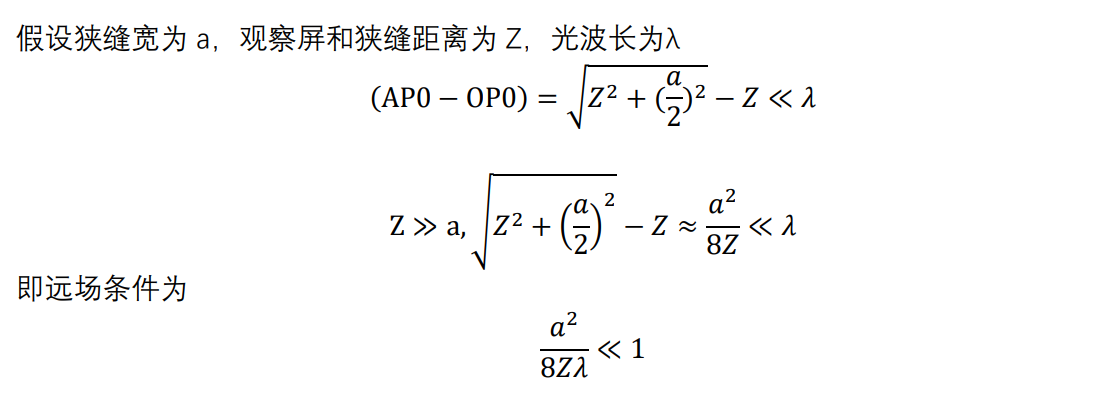
\includegraphics[width=0.8\textwidth]{attachments//illus-2.1.png}
\end{figure}
\subsubsection*{4. 采用数值计算的方法画出多种圆孔直径、多种观察屏和圆孔距离下的艾里斑图样。}
由公式$\Delta l = 1.22b\frac{\lambda}{D}$
\begin{figure}[htbp]
	\centering
	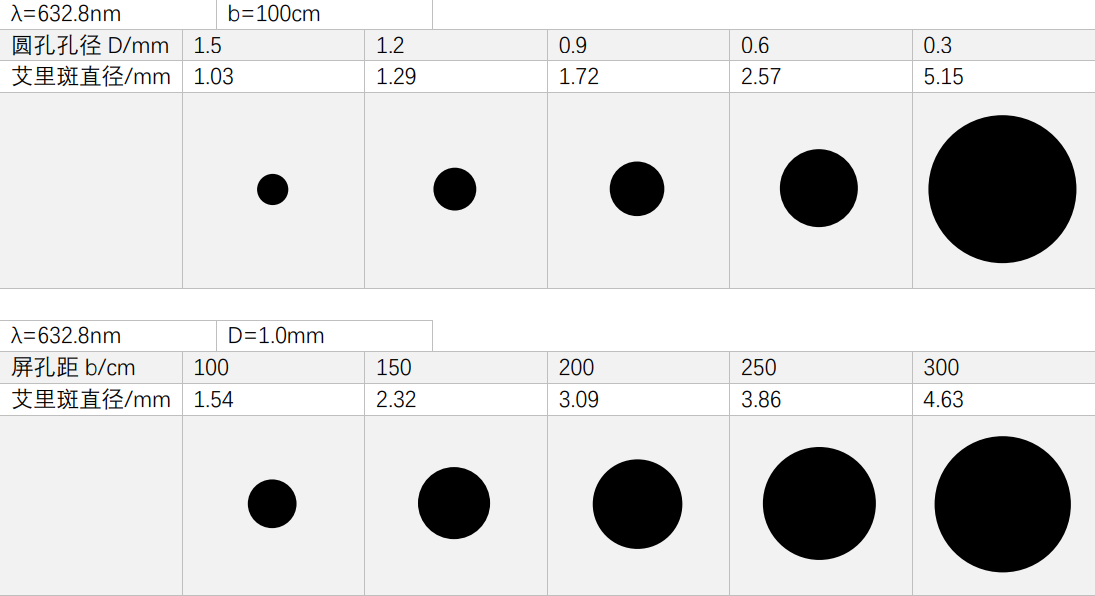
\includegraphics[width=0.8\textwidth]{attachments//illus-2.2.png}
\end{figure}


\end{document}

